\section{Diverses}
	\subsection{Frequenzgang zweier Systeme mit Rückkopplung }
			\begin{center}
        		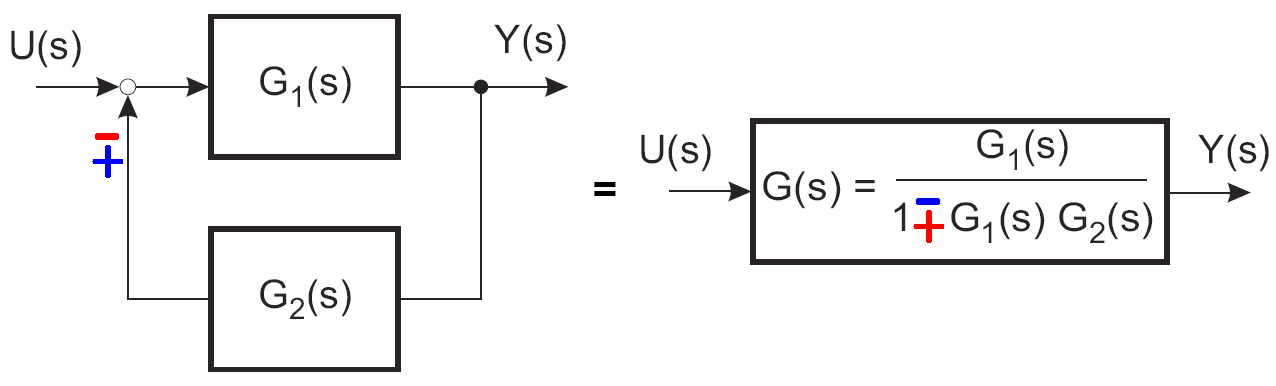
\includegraphics[height=3cm]{./bilder/feedback.png}
        	\end{center}

	\subsection{Graphisch Phasen-/Verstärkungsreserve}
		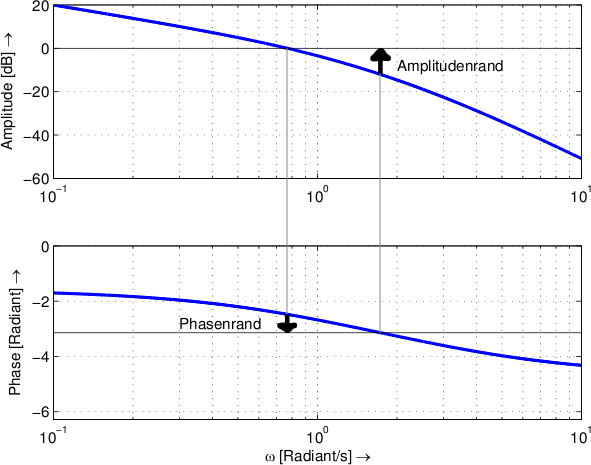
\includegraphics[width=7cm]{./bilder/bode-stabilitaet.png} \\
		Phasen-/Verstärkungsreserve = Phasen-/Amplitudenrand
		
		
%%%%%%%%%%%%%%%%%%%%%%%%%%%%%%%%%%%%%%%%%%%%%%%%%%%%%%%%%%%%%%%%%%%%%%%%%%%%%%%%%%%%%%%%%%%%
\newpage
	\subsection{Approximation des Bode-Diagramms}
	\renewcommand{\arraystretch}{1.5}
	\begin{tabular}{|p{4cm}|p{1.2cm}p{5cm}|p{1.2cm}p{4.5cm}|}
	\hline
	\textbf{UTF $H(s)$}
		& \textbf{Amplitude $|H(s)|$}
		&
		& \textbf{Phase $ \angle(H(s))$}
		& \\
	\hline
	\hline
	1) Konstanter Faktor & & & & \\
		$\alpha e^{j \beta}$
		& \parbox{1cm}{
			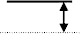
\includegraphics[width=1cm]{./bilder/bode-approx-konst.png}
		} 
		& Konst. $20 \log \alpha$
		& \parbox{1cm}{
			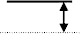
\includegraphics[width=1cm]{./bilder/bode-approx-konst.png}
		} 
		& Konst. $\beta$ \\
	\hline
	2) Pol im Ursprung & & & &\\
		$\frac{\alpha}{s}$
		& \parbox{1cm}{
			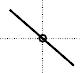
\includegraphics[width=1cm]{./bilder/bode-approx-ampl-tp-ord1.png}
		} 
		& \parbox{5cm}{
			Lin. Steigung $-20 db/Dek.$\\
			$0dB$ bei $\omega = \alpha$
		}
		& \parbox{1cm}{
			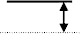
\includegraphics[width=1cm]{./bilder/bode-approx-konst.png}
		} 
		& Konst. $-\frac{\pi}{2}$ \\
	\hline
	3) Nullstelle im Ursprung & & & &\\
		$\alpha s$
		& \parbox{1cm}{
			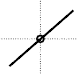
\includegraphics[width=1cm]{./bilder/bode-approx-ampl-hp-ord1.png}
		} 
		& \parbox{5cm}{
			Lin. Steigung $+20 db/Dek.$\\
			$0dB$ bei $\omega = \frac{1}{\alpha}$
		}
		& \parbox{1cm}{
			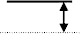
\includegraphics[width=1cm]{./bilder/bode-approx-konst.png}
		} 
		& Konst. $+\frac{\pi}{2}$ \\
	\hline
	4a) Reeller Pol & & & &\\
		$\frac{1}{s + \alpha}$
		& \parbox{1cm}{
			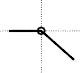
\includegraphics[width=1cm]{./bilder/bode-approx-ampl-4.png}
		} 
		& \parbox{5cm}{
			Konst. $-20 \log \alpha$ für $\omega < \alpha$\\
			dann Steigung $-20dB/Dek.$ 
		}
		& \parbox{1cm}{
			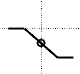
\includegraphics[width=1cm]{./bilder/bode-approx-phase-4.png}
		} 
		& \parbox{4.5cm}{
			Konst. $0$ für $\omega < \frac{\alpha}{10} $\\
			Konst. $-\frac{\pi}{2}$ für $\omega > 10 \alpha$
		}\\
	\hline
	4b) Reeller Pol &&&&\\
		$\frac{\alpha}{s + \alpha}$
		& \parbox{1cm}{
			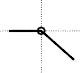
\includegraphics[width=1cm]{./bilder/bode-approx-ampl-4.png}
		} 
		& \parbox{5cm}{
			Konst. $0dB$ für $\omega < \alpha$\\
			dann Steigung $-20dB/Dek.$
		}
		& \parbox{1cm}{
			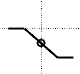
\includegraphics[width=1cm]{./bilder/bode-approx-phase-4.png}
		} 
		& \parbox{4.5cm}{
			Konst. $0$ für $\omega < \frac{\alpha}{10} $\\
			Konst. $-\frac{\pi}{2}$ für $\omega > 10 \alpha$
		}\\
	\hline
	5a) Reelle Nullstelle &&&& \\
		$s + \alpha$
		& \parbox{1cm}{
			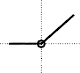
\includegraphics[width=1cm]{./bilder/bode-approx-ampl-5.png}
		} 
		& \parbox{5cm}{
			Konst. $20 \log \alpha$ für $\omega < \alpha$\\
			dann Steigung $+20dB/Dek.$
		}
		& \parbox{1cm}{
			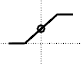
\includegraphics[width=1cm]{./bilder/bode-approx-phase-5.png}
		} 
		& \parbox{4.5cm}{
			Konst. $0$ für $\omega < \frac{\alpha}{10} $\\
			Konst. $+\frac{\pi}{2}$ für $\omega > 10 \alpha$
		}\\
	\hline
	5b) Reelle Nullstelle &&&& \\
		$\frac{s + \alpha}{\alpha}$
		& \parbox{1cm}{
			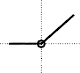
\includegraphics[width=1cm]{./bilder/bode-approx-ampl-5.png}
		} 
		& \parbox{5cm}{
			Konst. $0dB$ für $\omega < \alpha$\\
			dann Steigung $+20dB/Dek.$
		}
		& \parbox{1cm}{
			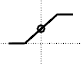
\includegraphics[width=1cm]{./bilder/bode-approx-phase-5.png}
		} 
		& \parbox{4.5cm}{
			Konst. $0$ für $\omega < \frac{\alpha}{10} $\\
			Konst. $+\frac{\pi}{2}$ für $\omega > 10 \alpha$
		}\\
	\hline
	\multicolumn{2}{|l}{6a) Konjugiert-komplexe Pole} &&& \\
		$\frac{1}{s^2+s\frac{\omega_p}{q_p}+\omega_p^2}$
		& \parbox{1cm}{
			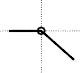
\includegraphics[width=1cm]{./bilder/bode-approx-ampl-6.png}
		} 
		& \parbox{5cm}{
			Konst. $-40 \log \omega_p$ für $\omega < \omega_p$\\
			dann Steigung $-40dB/Dek.$ für $\omega > \omega_p; -40 \log \omega_p$\\
			Überhöhung zwischen $\frac{\omega_p}{2}$, $\omega_p$ \& $2 \omega_p$\\
			Max. $20 \log \frac{q_p}{\omega_p^2}$ bei $\omega = \omega_p$
			}
		& \parbox{1cm}{
			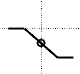
\includegraphics[width=1cm]{./bilder/bode-approx-phase-6.png}
		} 
		& \parbox{4.5cm}{
			Konst. $0$ für $\omega < \frac{\omega_p}{10^{\frac{1}{2q_p}}} $\\
			Konst. $-\pi$ für $\omega > \omega_p 10^{\frac{1}{2q_p}}$\\
			$-\frac{\pi}{2}$ bei $\omega = \omega_p$
		}\\
	\hline
	\multicolumn{2}{|l}{6b) Konjugiert-komplexe Pole} &&& \\
		$\frac{\omega_p^2}{s^2+s\frac{\omega_p}{q_p}+\omega_p^2}$
		& \parbox{1cm}{
			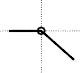
\includegraphics[width=1cm]{./bilder/bode-approx-ampl-6.png}
		} 
		& \parbox{5cm}{
			Konst. $0dB$ für $\omega < \omega_p$\\
			dann Steigung $-40dB/Dek.$ für $\omega > \omega_p; 0dB$\\
			Überhöhung zwischen $\frac{\omega_p}{2}$, $\omega_p$ \& $2 \omega_p$,
			Max. $20 \log q_p$ bei $\omega = \omega_p$
			}
		& \parbox{1cm}{
			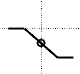
\includegraphics[width=1cm]{./bilder/bode-approx-phase-6.png}
		} 
		& \parbox{4.5cm}{
			Konst. $0$ für $\omega < \frac{\omega_p}{10^{\frac{1}{2q_p}}} $\\
			Konst. $-\pi$ für $\omega > \omega_p 10^{\frac{1}{2q_p}}$\\
			Bei $\omega = \omega_p$ genau $-\frac{\pi}{2}$
		}\\
	\hline
	\multicolumn{2}{|l}{7) Konjugiert-komplexe Nullstellen} &&& \\
		\parbox{4cm}{
			$s^2+s\frac{\omega_z}{q_z}+\omega_z^2$ \\ bzw. \\
			$\frac{s^2+s\frac{\omega_z}{q_z}+\omega_z^2}{\omega_z^2}$
		}
		& \multicolumn{2}{|p{6.2cm}|}{
			Analog zu 6a, 6b (jedoch Spiegelung an der 0dB-Linie)
		}
		
		& \multicolumn{2}{|p{6.2cm}|}{
			Analog zu 6a, 6b (jedoch Spiegelung an der 0 Grad-Linie)
		}\\
	\hline
	\multicolumn{5}{|p{18cm}|}{
		8) Serieschaltung von Systemen erfolgt durch \textbf{Superposition} der
		einzelnen Bode-Diagramme (Multiplikation von UTFs entspricht Addition im
		dB-Bereich). } \\
	\hline
	\end{tabular}
	\renewcommand{\arraystretch}{1}